\clearpage

\section{Vergleich Mesh Netzwerke}\label{sec:VergleichMeshNetzwerke}
Der Vergleich der Mesh-Netzwerke basiert auf den Messergebnissen die im Abschnitt \ref{sec:Messresultate} präsentiert wurden.
Die Messungen unterscheiden sich aufgrund der unterschiedlichen Messparameter, sowie dem Messaufbau (Wohnung/Labor/Haus).
Um einen Vergleich ziehen zu können, wird daher auf diese beiden Hauptmerkmale abgestellt.
Der Vergleich der Mesh Netzwerke, inkl. den wichtigsten Eigenschaften des Benchmarks, wurde in einem eigenständigen Paper im Anhang \ref{app:Paper} zusammengefasst.
Nachfolgend wird ein ausführlicher Vergleich der Mesh Netzwerke, bezüglich den oben genannten Hauptmerkmalen, präsentiert.
Im ersten Abschnitt \ref{subsec:VergleichMessreihen} werden die Messreihen und im zweiten Abschnitt \ref{subsec:VergleichTestumgebungen} die Testumgebungen verglichen.
Innerhalb dieser Abschnitte werden die Vergleichswerte gemäss Abschnitt \ref{subsubsec:Vergleichswerte} betrachtet.

\subsection{Vergleich der Messreihen}\label{subsec:VergleichMessreihen}
Dieser Vergleich bezieht sich auf eine gleichbleibende Testumgebung jedoch mit unterschiedlichen Messreihen.
Als Referenz wurde die Umgebung des Labors ausgewählt, da dort Messergebnisse aller Messreihen vorliegen (siehe Anhang \ref{app:MessprotokolleMeshBenchmark}).
Im Anschluss soll gezeigt werden, wie sich die einzelnen Mesh-Netzwerke bei ändernden Messreihen verhalten.

Zusammengefasst lassen sich die Messreihen folgendermassen unterscheiden (siehe auch Tabelle \ref{tab:MessungenMeshBenchmark}). 

\begin{itemize}
	\item Die \textbf{\textit{Payload}} wurde zwischen den Messreihen 1\&3, 2\&4 und 7\&8 von 8 Byte auf 32 Byte (BT Mesh), resp. 50 Byte (Thread, Zigbee) erhöht.
	\item  Der \textbf{\textit{Traffic Generation Mode}} wurde zwischen den Messreihen 1\&2 und 3\&4 von Random auf Sequentiell geändert.
	\item Die \textbf{\textit{Message-Dichte}} wurde zwischen den Messreihen 2\&7 und 4\&8 von 2.5 M/s (Messages/Sekunde auf 0.33 M/s gesenkt).
	\item Der \textbf{\textit{Disturbance}}-Vergleich kann zwischen der Messung 2 und der Messung 6 erfolgen. Bei Messung 6 ist die Disturbance eingeschaltet.
\end{itemize}

\subsubsection{Latenzzeit}\label{subsec:VergleichLatenzzeitMessreihen}
Durch die in Abbildung \ref{fig:Latenzzeiten_per_Hop_Messreihen} dargestellten Latenzzeiten wird ersichtlich, dass Bluetooth-Mesh am anfälligsten auf die Erhöhung der Payload reagiert. Eine detaillierte Analyse zu diesem Phänomen wird in Abschnitt \ref{subsubsec:FazitBluetoothMesh} durchgeführt. Die Verzögerung bleibt bei Zigbee und Thread trotz Erhöhung der Paketlänge stabil.

Eine Änderung des \textit{Traffic Generation Mode} von Random auf Sequentiell bewirkt bei Bluetooth-Mesh eine drastische Abnahme der Latenz. Bei Zigbee ist zwischen der Messreihe 1 und 2 ebenfalls eine Abnahme zu verzeichnen, welche jedoch nicht zwischen der Reihe 3 und 4 feststellbar ist. Somit muss ein anderer Einfluss für die Abnahme verantwortlich sein, welcher im Abschnitt \ref{subsubsec:FazitZigbee} behandelt wird.
Die Änderung des \textit{Traffic Generation Mode} führt bei Thread ebenfalls zu einer Verbesserung der Latenzzeiten.
Es zeigt sich, dass die Stacks mit gleichmässigem Nachrichtenaufkommen besser zurecht kommen, als mit zufällig generierter Abfolge der Nachrichten.

Das Senken der Message Dichte bewirkt bei Bluetooth-Mesh eine markante Abnahme der Latenzzeit.
Bei Thread und Zigbee bleibt die Latenz nahezu konstant.
 
Die Einbringung von Störungen hat lediglich bei Bluetooth-Mesh einen negativen Einfluss, wodurch sich die Latenzzeit erhöht.
Dank CSMA\slash CA des \textit{IEEE 802.15.4} MAC Layers, werden die Messungen von Thread und Zigbee nicht beeinflusst.

\begin{figure}[H]
	\centering
	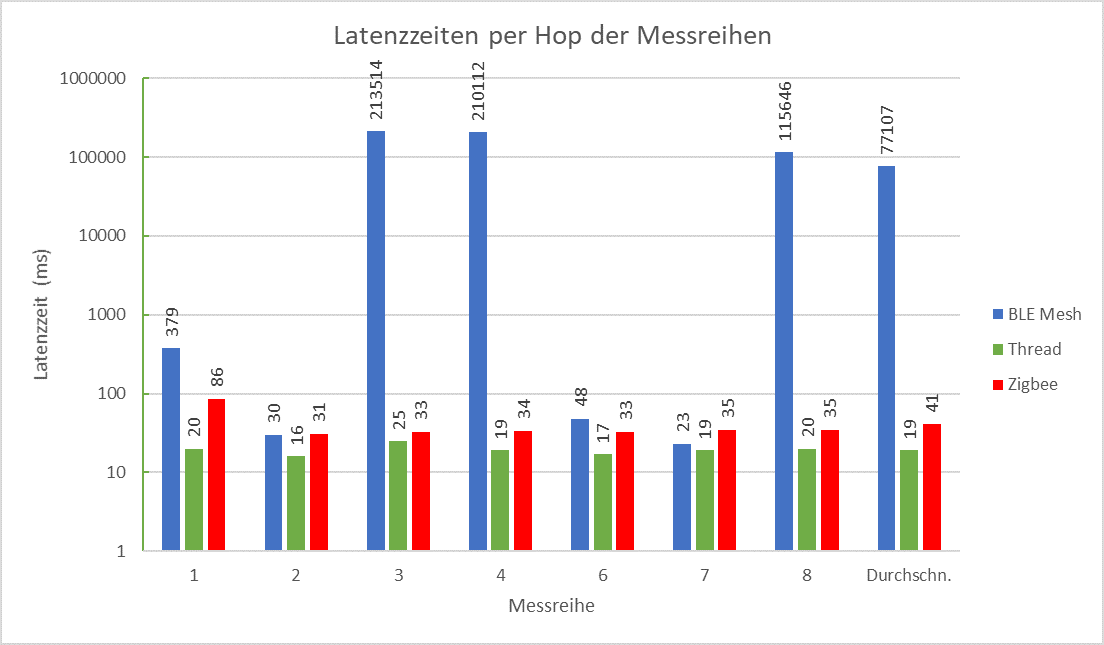
\includegraphics[width=1.0\textwidth]{Latenzzeiten_per_Hop_Messreihen.png}
	\caption{Durchschnittliche Latenzzeit per Hop der einzelnen Messreihen im Vergleich}\label{fig:Latenzzeiten_per_Hop_Messreihen}
\end{figure}

\subsubsection{Durchsatz}\label{subsec:VergleichDurchsatzMessreihen}

Die in Abbildung \ref{fig:Durchsätze_per_Hop_Messreihen} dargestellten Durchsatzraten zeigen, dass sich ähnliche Vergleichsresultate ergeben wie bei der Latenzzeit zuvor.
Bluetooth-Mesh reagiert am anfälligsten auf die Payload-Erhöhung. Wie bereits in Abschnitt \ref{subsec:VergleichLatenzzeitMessreihen} dargelegt wird eine detaillierte Analyse zu diesem Phänomen in Abschnitt \ref{subsubsec:FazitBluetoothMesh} durchgeführt. Der Durchsatz steigt bei Zigbee und Thread durch die Erhöhung der Paketlänge stark an. Dies wird in Abschnitt \ref{subsubsec:FazitThread} für Thread und in Abschnitt \ref{subsubsec:FazitZigbee} für Zigbee genauer untersucht.

Eine Änderung des \textit{Traffic Generation Mode} von Random auf Sequentiell bewirkt bei Bluetooth-Mesh eine drastische Zunahme des Durchsatzes.
Bei Thread ist ebenfalls eine Steigerung der Übertragungskapazität feststellbar.
Bei Zigbee hingegen bewirkt diese Änderung keine merkliche Verbesserung des Durchsatzes.

Die Senkung der Message-Dichte führt bei Bluetooth-Mesh zu einer Verbesserung des Durchsatzes. Bei Thread und Zigbee kann keine Abhängigkeit festgestellt werden.

Das Einbringen von Störungen hat bei allen Netzwerken einen leicht negativen Einfluss, wodurch der Durchsatz sinkt. 

\begin{figure}[H]
	\centering
	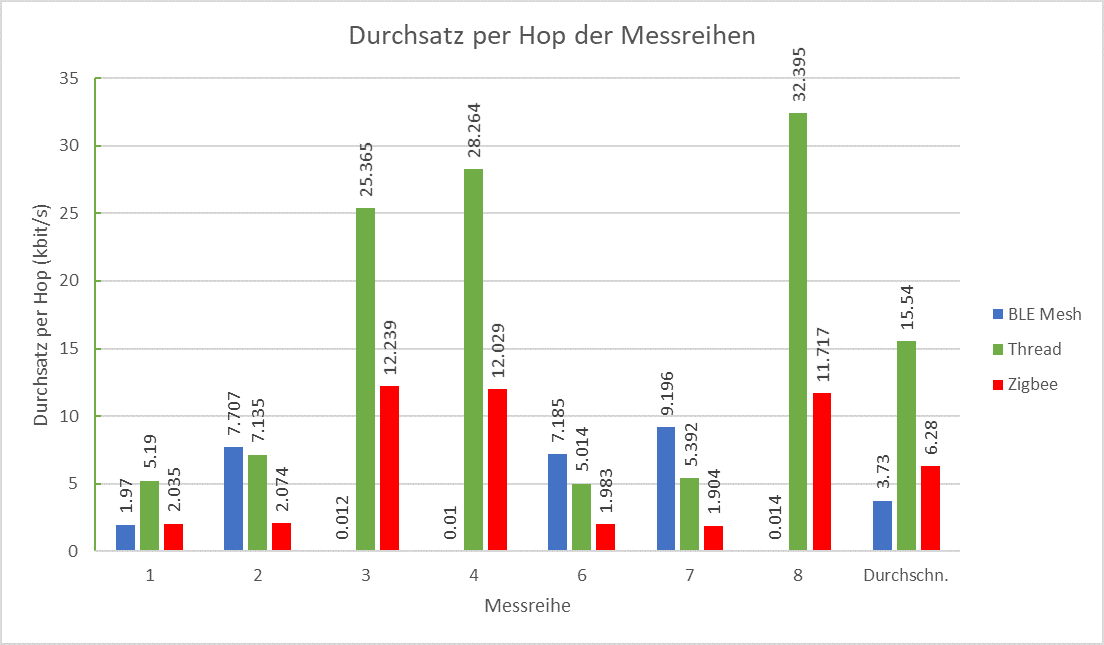
\includegraphics[width=1.0\textwidth]{Durchsatz_per_Hop_Messreihen.png}
	\caption{Durchschnittlicher Durchsatz per Hop der einzelnen Messreihen im Vergleich}\label{fig:Durchsätze_per_Hop_Messreihen}
\end{figure}

\subsubsection{Paketverlust}\label{subsec:VergleichPaketverlustMessreihen}
Bei der Betrachtung des Paketverlustes, zeigt sich Bluetooth-Mesh sehr anfällig auf die Erhöhung der Paketlänge.
Die Abbildung \ref{fig:{fig:PaketverlusteMessreihen}} zeigt dies deutlich.
In Abschnitt \ref{subsubsec:FazitBluetoothMesh} wird diese Problematik genauer untersucht.
Zigbee und Thread zeigen sich über alle Messreihen hinweg, sehr konstant und zuverlässig.
Das CSMA\slash CA des \textit{IEEE 802.15.4} MAC Layers erweist sich auch hier als sehr nützlich.


\begin{figure}
	\centering
	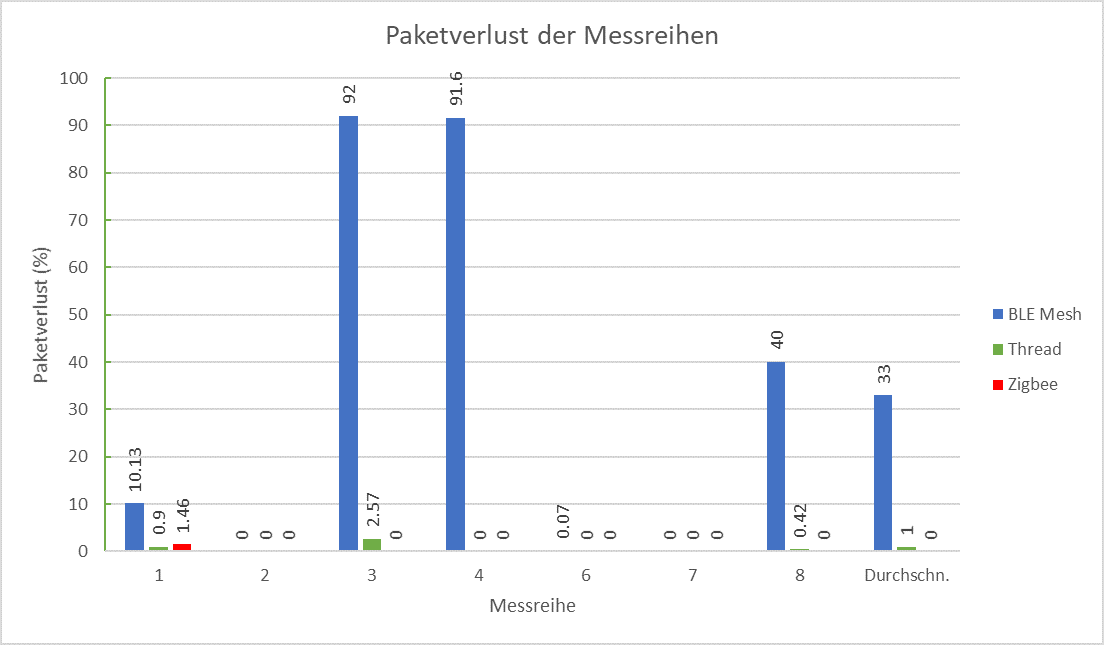
\includegraphics[width=1.0\textwidth]{Paketverlust_Messreihen.png}
	\caption{Durchschnittlicher Paketverlust der einzelnen Messreihen im Vergleich}\label{fig:PaketverlusteMessreihen}
\end{figure}

\subsubsection{Energieverbrauch}\label{subsec:VergleichEnergieverbrauchMessreihen}
Durch Abbildung \ref{fig:EnergieverbrauchMessreihen} wird ersichtlich, dass Bluetooth-Mesh den etwas geringeren Energiebedarf aufweist als Thread und Zigbee. Ansonsten zeigen alle Netzwerke ähnliche Resultate unabhängig der Messreihen.
Die Unterschiede zwischen den Protokollen fallen sehr gering aus.
Es kann also kein wesentlicher Unterschied bezüglich Energiebedarf festgestellt werden.
\todo{Raffi: Wieso sind die Werte bei den Messungen 7 und 8 höher als beim Rest? Können wir das begründen?} 

\begin{figure}[H]
	\centering
	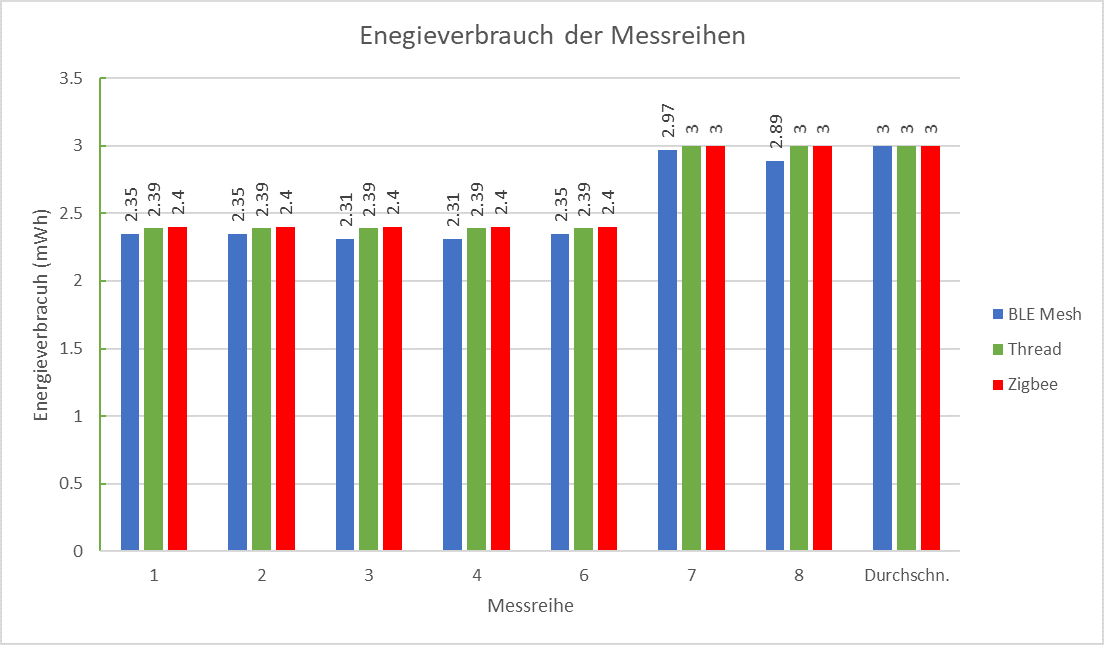
\includegraphics[width=1.0\textwidth]{Energieverbrauch_Messreihen.png}
	\caption{Durchschnittlicher Energiebedarf der einzelnen Messreihen im Vergleich}\label{fig:EnergieverbrauchMessreihen}
\end{figure}


\subsection{Vergleich Testumgebungen}\label{subsec:VergleichTestumgebungen}

Der nachfolgende Vergleich bezieht sich auf eine gleichbleibende Messreihe, welche in unterschiedlichen Testumgebungen durchgeführt wurde.
Als Referenz wurde die Messreihe 2 ausgewählt, da diese für alle Testumgebung repräsentative Resultate aufweist (siehe Anhang \ref{app:MessprotokolleMeshBenchmark}).
Im Anschluss wird gezeigt, wie sich die Resultate der einzelnen Mesh-Netzwerke bei wechselnden Testumgebungen verändern.

\subsubsection{Latenzzeit}\label{subsec:VergleichLatenzzeitTestumgebungen}
Abbildung \ref{fig:Latenzzeiten_per_Hop_Testumgebungen} zeigt, dass die Testumgebung Labor bei allen Netzwerken die geringsten Latenzzeiten verursacht.
Bluetooth-Mesh erfährt bei flächenmässig weiter Verteilung der Teilnehmer, wie sie im Haus anzutreffen ist, die grösste Steigerung der Latenzzeit. Zigbee weist in der Wohnung eine kaum relevante Erhöhung der Verzögerung auf und Thread zeichnet sich als unabhängig bezüglich der Testumgebung aus. 

\begin{figure}[H]
	\centering
	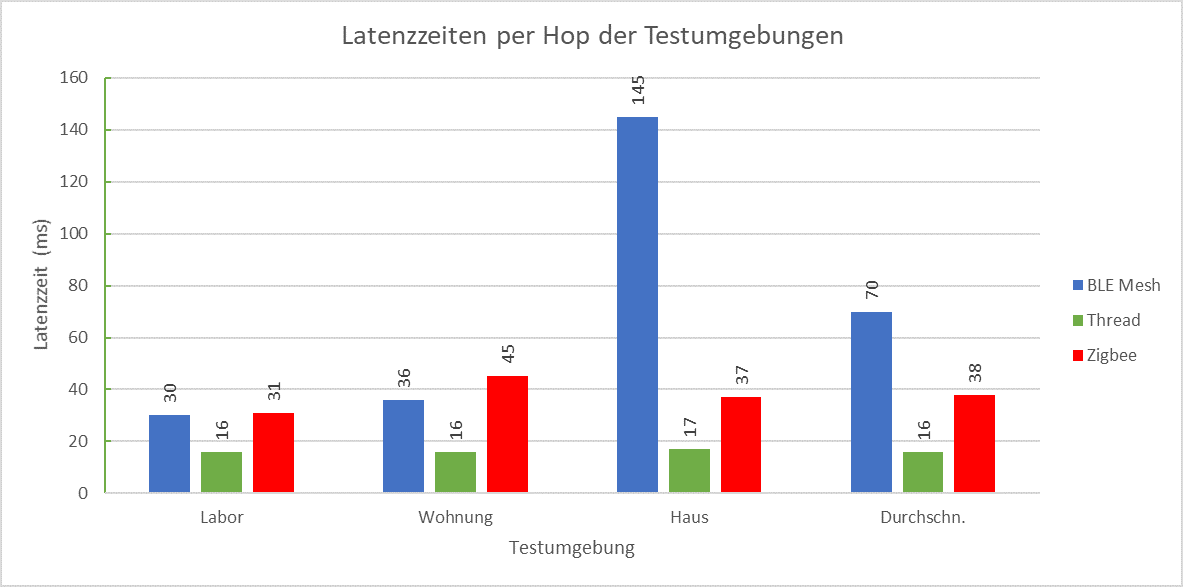
\includegraphics[width=1.0\textwidth]{Latenzzeiten_per_Hop_Testumgebungen.png}
	\caption{Durchschnittliche Latenzzeit per Hop der einzelnen Testumgebungen im Vergleich}\label{fig:Latenzzeiten_per_Hop_Testumgebungen}
\end{figure}

\subsubsection{Durchsatz}\label{subsec:VergleichDurchsatzTestumgebungen}
Ähnlich zu den Betrachtungen der Latenzzeit zeigt Abbildung \ref{fig:Durchsätze_per_Hop_Testumgebungen} den höchsten Durchsatz im Testaufbau Labor.
Bluetooth-Mesh erfährt hingegen, den grössten Einfluss durch die Änderung der Topologie. 

\begin{figure}[H]
	\centering
	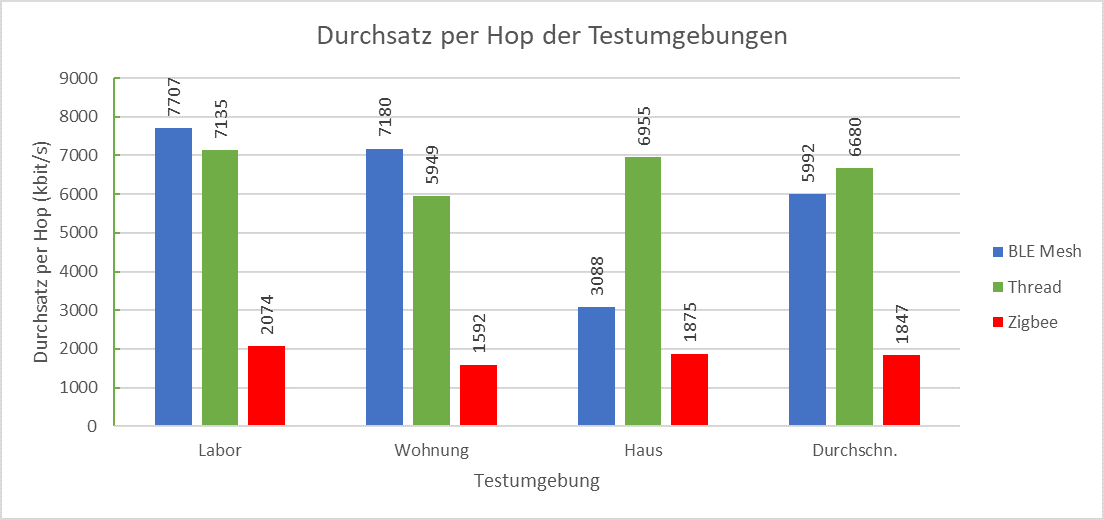
\includegraphics[width=1.0\textwidth]{Durchsatz_per_Hop_Testumgebungen.png}
	\caption{Durchschnittlicher Durchsatz per Hop der einzelnen Testumgebungen im Vergleich}\label{fig:Durchsätze_per_Hop_Testumgebungen}
\end{figure}

\subsubsection{Paketverlust}\label{subsec:VergleichPaketverlustTestumgebungen}
Abbildung \ref{fig:Durchsätze_per_Hop_Testumgebungen} zeigt, dass im Labor-Aufbau alle Netzwerke zuverlässig und konstant arbeiten.
In der Wohnung erlebt Bluetooth-Mesh einen geringen Anstieg des Paketverlusts während die Änderung bei Thread kaum relevant ist.
Zigbee zeigt gar keine Veränderung der Paketverlustrate.
Bei starker Verzweigung des Netzwerkes, wie dies im Haus der Fall ist, weisen alle Netzwerke einen Anstieg der Verlustrate auf.


\begin{figure}[H]
	\centering
	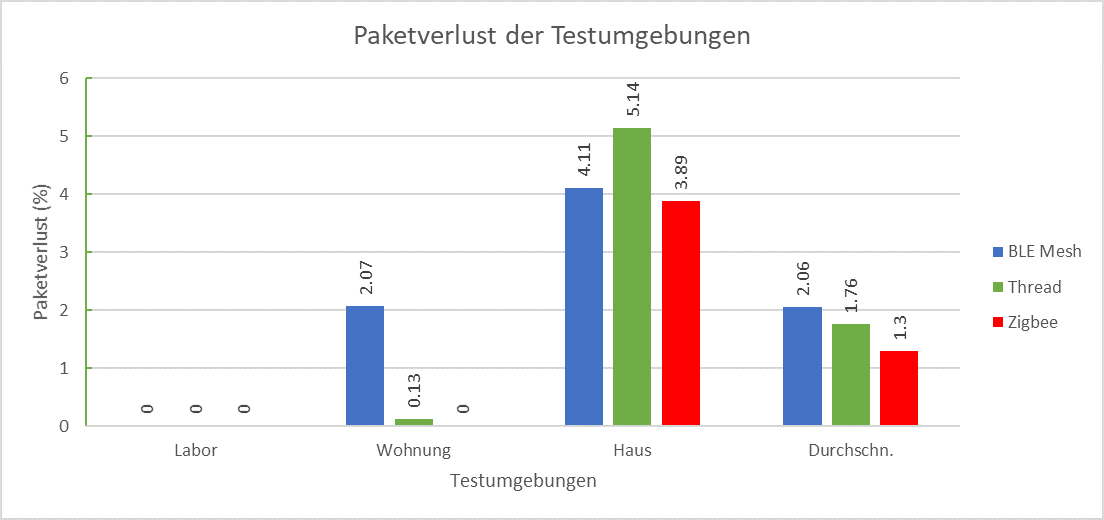
\includegraphics[width=1.0\textwidth]{Paketverlust_Testumgebungen.png}
	\caption{Durchschnittlicher Paketverlust der einzelnen Testumgebungen im Vergleich}\label{fig:PaketverlusteTestumgebungen}
\end{figure}

\subsection{Fazit}\label{subsec:FazitVergleich}
Alle Mesh-Netzwerke mussten diversen Tests standhalten. Die Ergebnisse aus den Messreihen 1 bis 4 aus allen Testumgebungen wurden als Durchschnittswert zusammengefasst, um einen finalen Vergleich zu erzielen. Abbildung \ref{fig:Messresultate_Fazit} zeigt alle Ergebnisse auf einen Blick.

\begin{figure}[H]
	\centering
	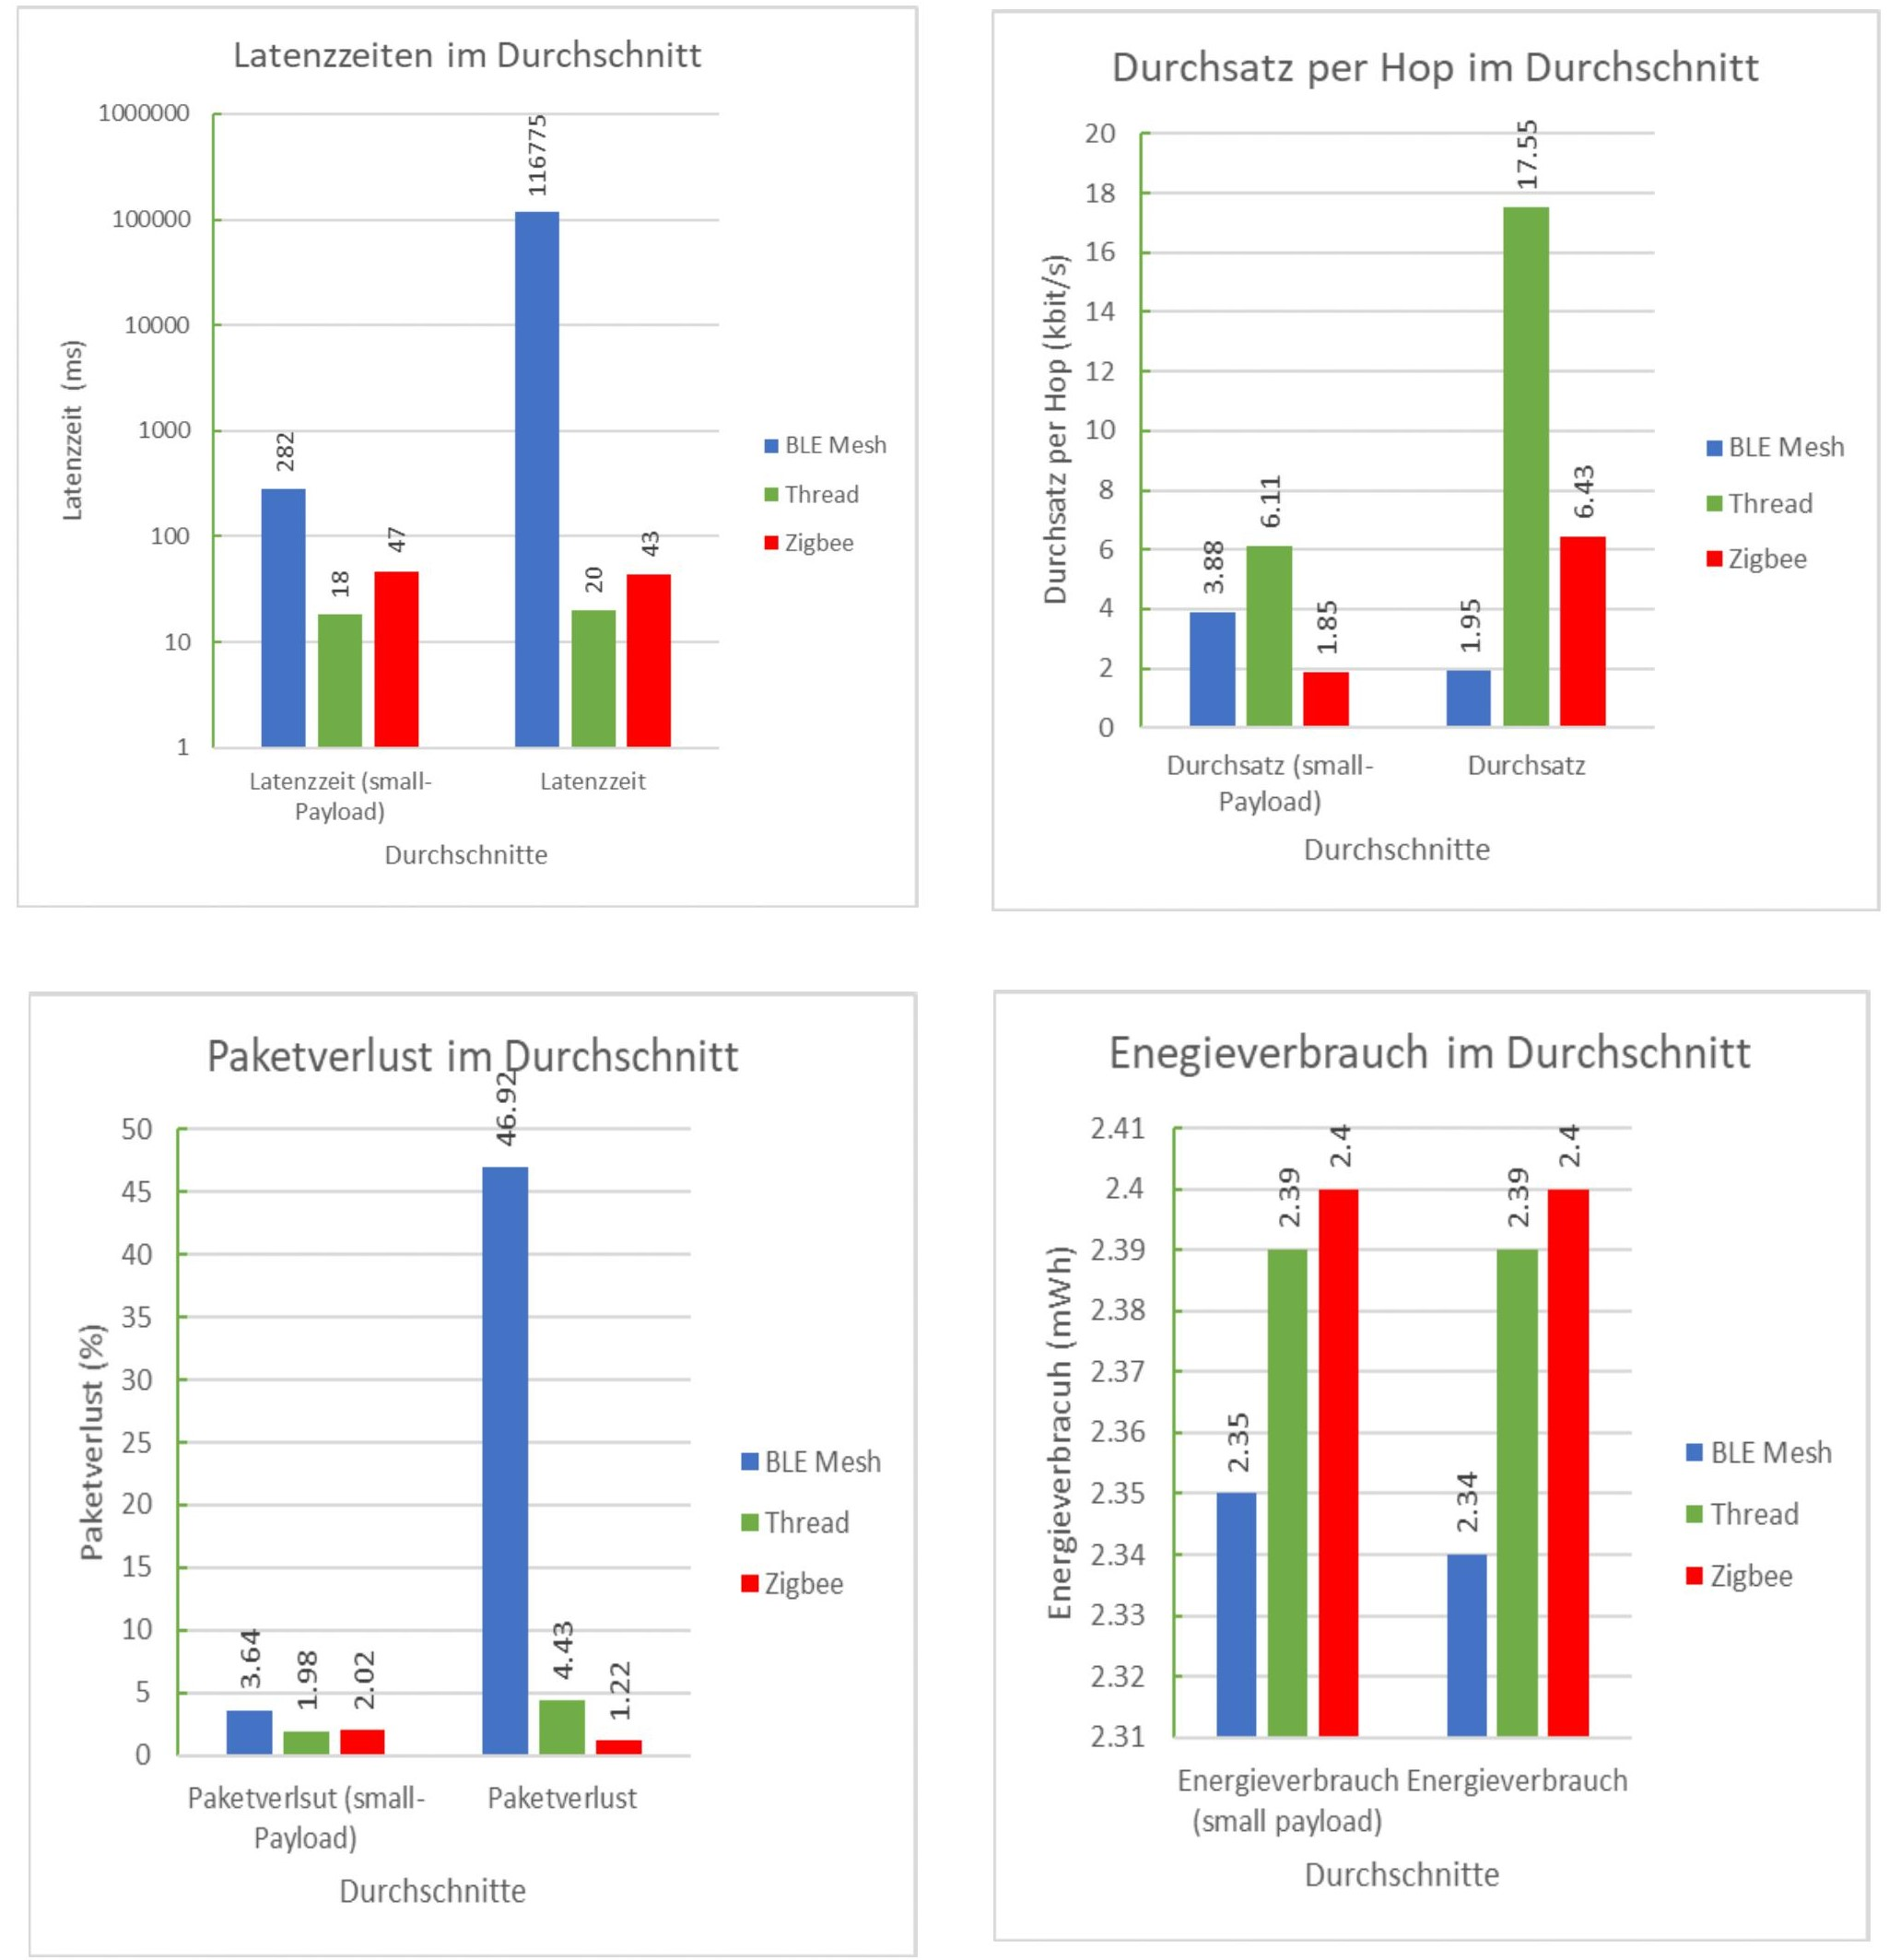
\includegraphics[width=1.0\textwidth]{Messresultate_Fazit.jpg}
	\caption{Durchschnittliche Messgrössen im Vergleich inkl. separater Betrachtung der Messergebnisse, welche mit 8-Byte Paketlänge erzielt wurden}\label{fig:Messresultate_Fazit}
\end{figure}

Thread geht shliesslich als klarer Sieger hervor.
Dieser Netzwerk-Stack hat die Tests mit den besten Ergebnissen absolviert.
Auf dem zweiten Platz steht Zigbee, welches mit seiner konstanten Latenz und als zuverlässigstes Protokoll die Daten verarbeiten konnte.
Dabei gilt zu beachten, dass bei Zigbee die Anzahl Hops nicht berücksichtigt wurden (siehe Abschnitt \ref{subsec:Validierung}), was zu einer leichten Verfälschung der Ergebnisse führt.
Bluetooth-Mesh kann zwar durch den niedrigen Energiebedarf brillieren, schneidet jedoch in Sachen Performance deutlich schlechter ab als seine Konkurrenten Thread und Zigbee.
Im Anschluss wird jedes Protokoll genauer analysiert und auf die Vor- und Nachteile sowie mögliche Verbesserungen eingegangen. 


\subsubsection{Thread}\label{subsubsec:FazitThread}
Wie aus den vorhergehenden Kapiteln ersichtlich, hat der Thread Stack die Messungen mit den besten Ergebnissen abgeschlossen.
Das bedeutet aber nicht unbedingt, dass der Stack der Beste ist.
Es ist klar zu erkennen, dass der Thread Stack dank seiner automatischen Bestimmung von Routing-Knoten, sich seiner Umgebung gut anpassen kann.
Die Latenzzeit der gesendeten Nachrichten ändert sich in verschiedenen Umgebungen nur minimal.
Das bedeutet, dass sich der Thread Stack sehr gut für eine Hausautomation eignet.
Wenn sich Sensoren oder Aktoren verschieben, z.B. wenn eine Lampe einen neuen Standort erhält, erkennt dies der Stack und kann das Routing der Knoten anpassen.
Da sich das Netz sehr gut erweitern lässt und sich die Latenzzeiten eher tief zeigen, kann das Thread Netzwerk ausserdem gut für Industrieanwendungen verwendet werden. 

Durch das automatische Routen der Knoten entsteht auf den einzelnen Nodes jedoch ein Overhead, der zum Beispiel BT Mesh nicht aufweist.
Aus diesem Grund ist der Energieverbrauch auf den Knoten höher, was sich auch in Abbildung \ref{fig:EnergieverbrauchMessreihen} zeigt. Dies ist zwar keine repräsentative Messung, da nur die aktiven Radio Zeiten gemessen wurden. Dennoch kann es die vorherige These mit dem Overhead bestätigen. 

Anders als bei BT-Mesh können mit dem IEEE 802.15.4 und dem 6LoWPAN Layer grössere Pakete versendet werden. Das bedeutet, dass die Segmentierung im Gegensatz zu BT Mesh später stattfindet. Dies erklärt das Phänomen, dass sich der Durchsatz mit steigender Payload vergrössert. Der Thread Stack erreicht bei manchen Messreihen einen Durchsatz von bis zu 32 kbit pro Sekunde. Dies ist jedoch eher unwahrscheinlich. Da bei den Durchschnittsberechnungen kein Median verwendet wurde, können Extremwerte den Durchschnitt verfälschen. Es gab sehr wenige Latenzmessungen, die fehlerhaft waren und eine Latenz unter 0.5ms aufwiesen. Durch diesen Fehler wurde der Durchsatz in der Auswertung unwahrscheinlich hoch. 

\subsubsection{Zigbee}\label{subsubsec:FazitZigbee}
Die Resultate und Vergleiche aus den vorhergehenden Abschnitten zeigen, dass das Zigbee Protokoll in dieser Implementation eine solide Performance abliefert.
Auch wenn Zigbee nicht ganz an jene Leistung von Thread herankommt, zeigen die Ergebnisse wieso Zigbee zurzeit das am weitest verbreitete WPAN Protokoll ist.

Die durchschnittlichen Latenzzeiten liegen zwischen 30ms und 50ms. Damit schneidet Zigbee besser als Bluetooth ab, jedoch liegen die Ergebnisse hinter jenen Durchschnittswerten von Thread.
Dies kommt nicht allzu überraschend.
Sehr interessant zu beobachten sind die Verteilungen der Latenzzeiten, wie sie beispielsweise in Abbildung \ref{fig:VerteilungderLatenzzeiten} zu sehen sind.
Anders als Thread weist Zigbee dort deutliche Peaks bei 40ms und 70ms auf.
Diese Beobachtung kann bei sämtlichen Messresultaten gemacht werden.
Ausreisser nach unten gibt es praktisch keine und solche nach oben nur sehr vereinzelt.
Es kann also festgestellt werden, dass bei Zigbee mit einer minimalen Latenzzeit von ca. 30ms gerechnet werden muss, diese Schwelle aber in den seltensten Fällen deutlich überschritten wird.
Zigbee wäre also auch für eher zeitkritische Anwendungen geeignet, da die Latenzzeiten deterministisch sind.
In diesen Zusammenhang nochmals zu erwähnen ist, dass die Information über die Anzahl Hops die ein Paket passiert hat, leider nicht erfasst werden konnte (siehe Abschnitt \ref{subsec:ZigbeeSchwierigkeitenbeiderUmsetzung}).
Es kann davon ausgegangen werden, dass der Peak bei 70ms in den Latenzzeiten, diesem Problem verschuldet ist.
Wenn also die Anzahl Hops erfasst werden könnten, dürfte sich die Verteilung der Latenzzeiten wohl nochmals reduzieren und die Ergebnisse würden noch besser ausfallen.

Die Ergebnisse aus Abbildung \ref{fig:Latenzzeiten_per_Hop_Messreihen} zeigen eine weitere interessante Eigenschaft von Zigbee.
In Messreihe 1 beträgt die durchschnittliche Latenzzeit von 86ms mehr als das Doppelte der Durchschnittswerte in den übrigen Messreihen.
Die Ursache dafür kann nicht abschliessend geklärt werden.
Jedoch liegt die Vermutung nahe, dass sich das Mesh Netz während dieser Messreihe noch nicht komplett aufgebaut respektive das \textit{Commissioning} und \textit{Route Discovery} noch nicht abgeschlossen war.
Dies verursachte zusätzlichen Traffic und beeinflusste den Benchmark.

Auffallend tief ist auch der Paketverlust.
In den meisten Fällen lag dieser sogar bei 0 Prozent.
Hier macht sich das CSMA\slash CA des \textit{IEEE 802.15.4} MAC Layers bemerkbar.
Zudem wirkt sich hier wohl die Unicast Adressierung innerhalb von Zigbee positiv aus.
Die Gesamtbelastung des Netzes kann dadurch deutlich minimiert werden.

Die Erhöhung der Payload von 8 auf 50 Byte hat die Latenzzeiten bei den Zigbee Messungen nicht merklich beeinflusst.
Dies bewirkt, dass der Durchsatz mit grösserer Payload zunimmt.
Da die Segmentierung dank \textit{IEEE 802.15.4} erst ab 127 Byte Framelänge startet, ist dies auch nicht weiter verwunderlich.
Gegenüber BT-Mesh haben Zigbee wie auch Thread den klaren Vorteil grössere Payloads versenden zu können, ohne segmentieren zu müssen.

Zigbee brilliert in den Anwendungen, in denen es bereits verbreitet eingesetzt wird.
Beispielsweise eine komplette Hausautomation oder eine einfachere Lichtsteuerung.
Bis zu einer Netzwerkgrösse von ungefähr 200 Nodes mit einigermassen kleinem Verkehrsaufkommen ist Zigbee die ideale Wahl.
Ergänzt durch die \textit{Zigbee Cluster Library} welche die Systeme herstellerunabhängig macht wird Zigbee noch interessanter.


\subsubsection{Bluetooth Mesh}\label{subsubsec:FazitBluetoothMesh}
Die Performance von Bluetooth-Mesh ist stark von der Belastung abhängig, wie aus Abschnitt \ref{subsec:VergleichMessreihen} zu erkennen ist.
Der grösste Einfluss auf die Performance hatte die Länge der gesendeten Nachrichten.
Ursach dafür ist, dass ein einzelnes Bluetooth-Mesh-Paket lediglich 10-Byte Payload aufnehmen kann (siehe Abschnitt \ref{subsec:BLEMeshStack})\todo{Raffi: Verweis falsch}. Der Stack beginnt mit der Segmentierung der Daten in mehrere kleine Pakete. Bei 32-Byte sind dies bereits 4 Frames. Damit ist der Network-Stack überfordert. 

\begin{figure}[H]
	\centering
	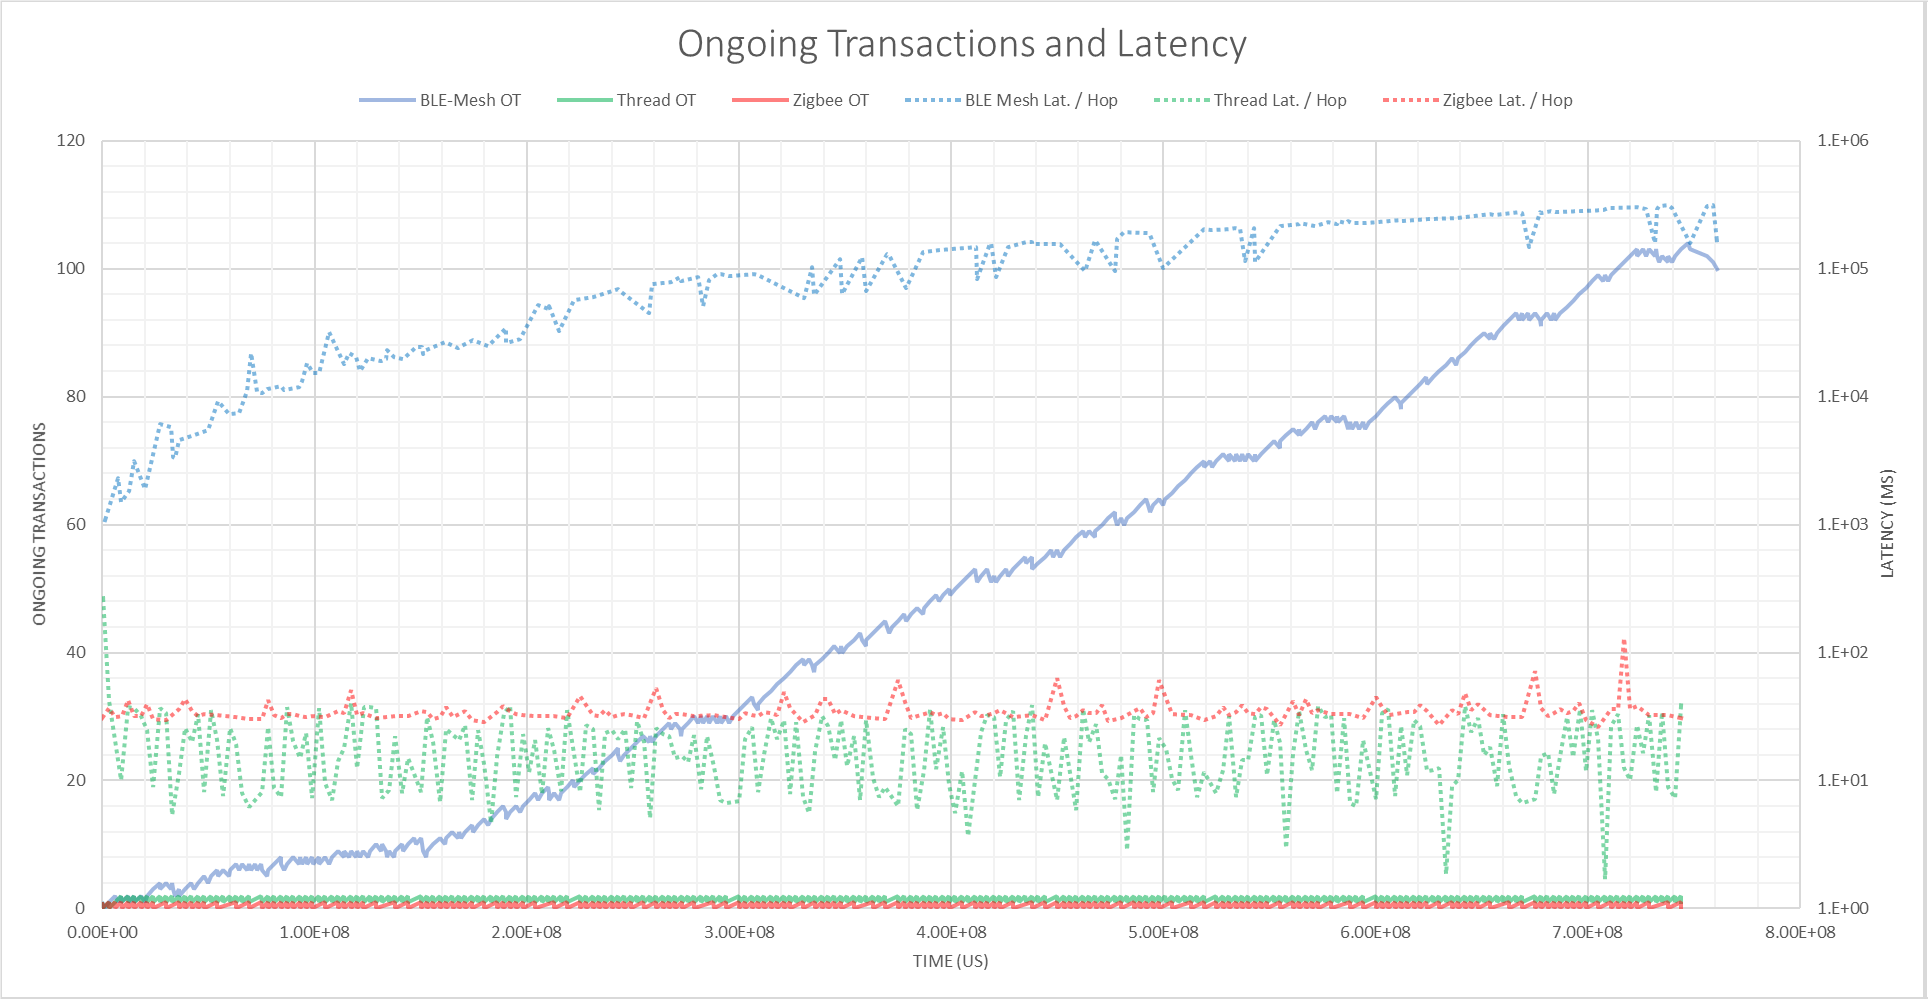
\includegraphics[width=1.0\textwidth]{Bluetooth_Mesh_Big_Payload_Issue.png}
	\caption{Ongoing Transactions und Latenzzeiten einer Messung mit 32Byte Paketlänge}\label{fig:Bluetooth_Mesh_Big_Payload_Issue}
\end{figure}

Abbildung \ref{fig:Bluetooth_Mesh_Big_Payload_Issue} zeigt eine Messung mit 32-Byte Payload bei einer Message-Dichte von 3 Sekunden/Message, welche sequentiell versendet wurden.
Dabei ist zu erkennen, dass die Anzahl der Ongoing Transactions immer weiter ansteigt.
Erst in der Nachtbearbeitungszeit sinkt die Kurve wieder.
Dies deutet darauf hin, dass zu viel Traffic im Netz vorhanden ist. In Korrelation mit den Ongoing Transactions steigt die Latenz von einer Sekunde auf einige 100 Sekunden an.

Vermutlich entsteht eine zu hohe Message-Dichte, da zu viele Relay-Nodes die empfangenen Messages wiederholen. Durch deaktivieren einiger Relays könnte der Netzaufbau entlastet werden. Jedoch erfordern solche manuellen Eingriffe Fachwissen und verringern die Ausfallsicherheit des Netzes. 







